\section{System Design}
\label{sec-design}

In this section, we present a detailed description of our wireless
sensor array for volcanic monitoring. Our initial experiment focused on
establishing feasibility by capturing complete, 
high-resolution signals from a small number of wireless sensor nodes, 
and comparing this data to that from a colocated wired station. 
However, our system architecture can generalize to much larger
deployments, as we describe in Section~\ref{sec-distrib}.

\subsection{System architecture}

\begin{figure*}[t]
\begin{center}
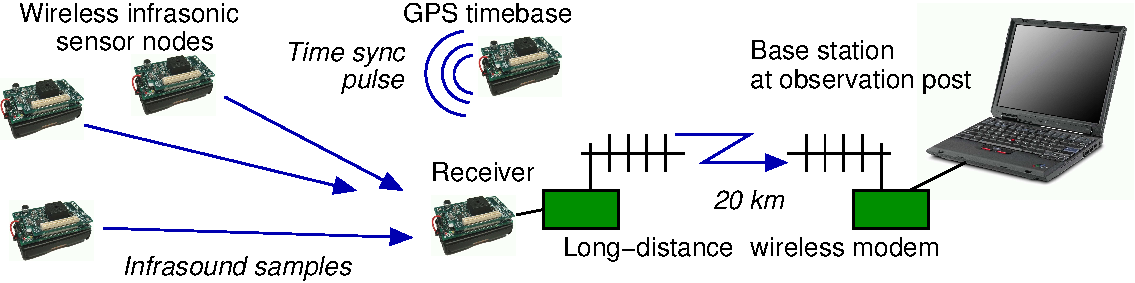
\includegraphics[width=0.9\hsize]{./figures/schematic.pdf}
\end{center}
\caption{\small {\bf System architecture of the infrasonic sensor
array.}}
\label{fig-arch}
\end{figure*}

Our design consists of several components, shown
in Figure~\ref{fig-arch}. The first is a set of {\em infrasound
monitoring nodes}, which sample low-frequency acoustic signals (up to
50~Hz). These nodes transmit their signals to an {\em aggregator node},
which relays the signals over a long-distance wireless link to a {\em
wired base station}, a laptop running various
software tools to visualize, store, and analyze the real-time signals
from the wireless array. To establish a common time base across the
captured signals, a {\em GPS receiver node} is used, which receives a
GPS time signal and relays the data to the infrasound and aggregator
nodes through radio messages.  

The infrasound, aggregator, and GPS receiver
nodes are based on the Mica2 mote, a typical wireless sensor device. It
consists of a 7.3~MHz ATmega128L processor, 128KB of code memory, 4KB of
data memory, and a Chipcon CC1000 radio operating at 433~MHz with a data
rate of approximately 34~Kbps. The Mica2 runs a lean, component-oriented
operating system, called TinyOS~\cite{tinyos-asplos00}.

\subsection{Infrasound node}

\begin{figure*}[t]
\centering
\subfigure[][Infrasonic monitoring node.]{
  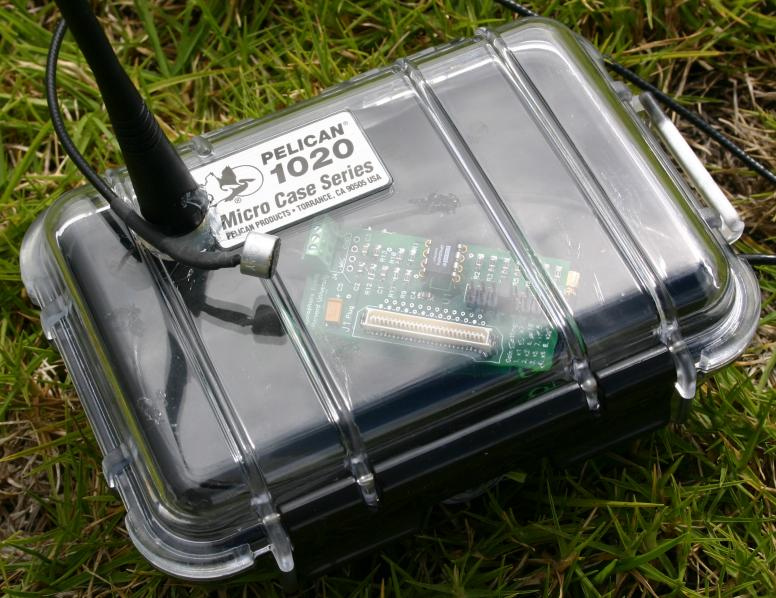
\includegraphics[height=0.1\vsize]{./figures/pics/volcanomote3-small.jpg}
}
\qquad
\subfigure[][FreeWave modem.]{
  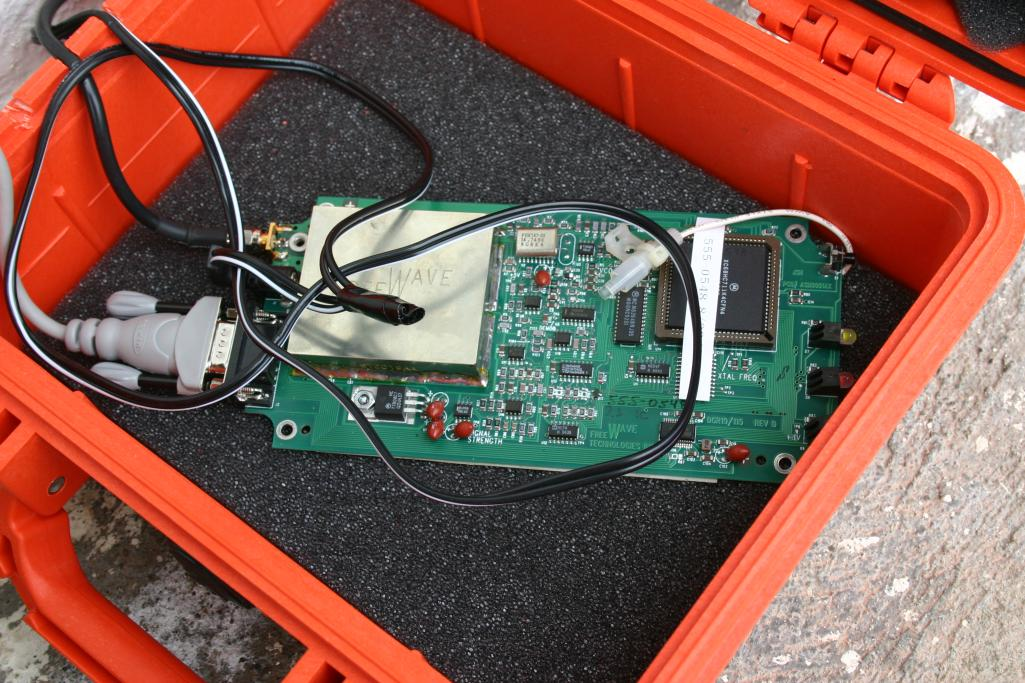
\includegraphics[height=0.1\vsize]{./figures/pics/freewave.jpg}
}
\qquad
\subfigure[][Yagi antenna oriented towards observatory.]{
  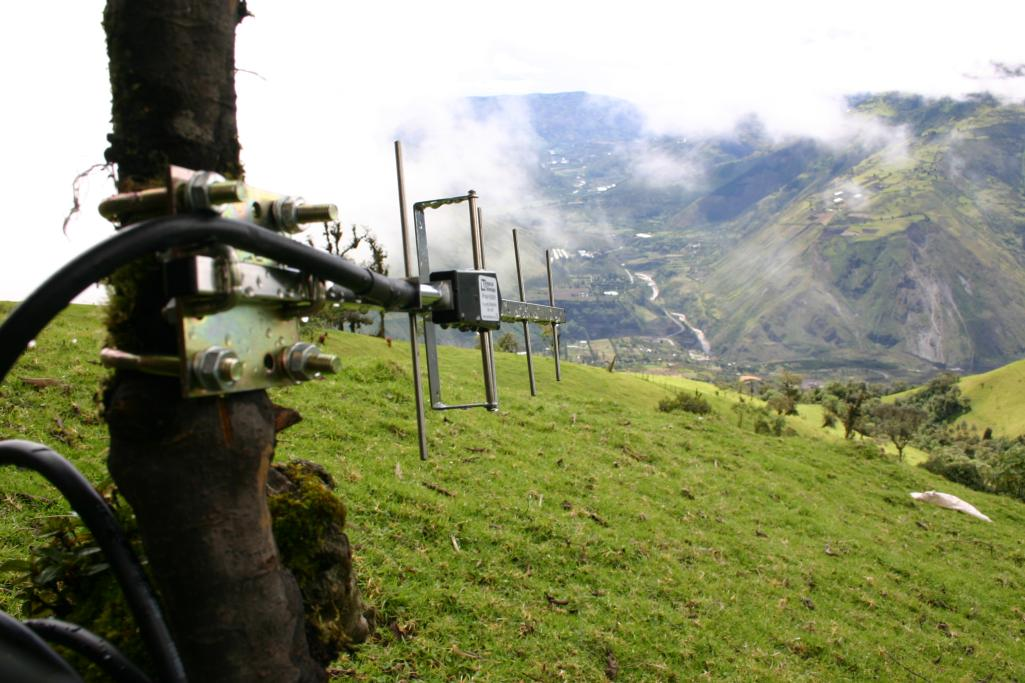
\includegraphics[height=0.1\vsize]{./figures/pics/yagi.jpg}
}
\caption{\small {\bf Equipment used in our sensor network deployment.}}
\label{fig-infrasound}
\end{figure*}
%\begin{figure*}[t]
%\begin{center}
%\begin{tabular}{ccc}
%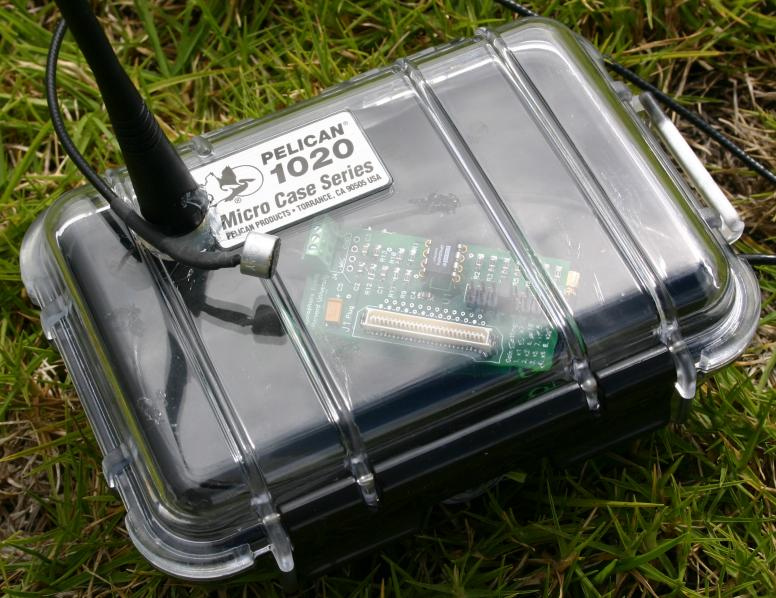
\includegraphics[height=0.1\vsize]{./figures/pics/volcanomote3-small.jpg} &
%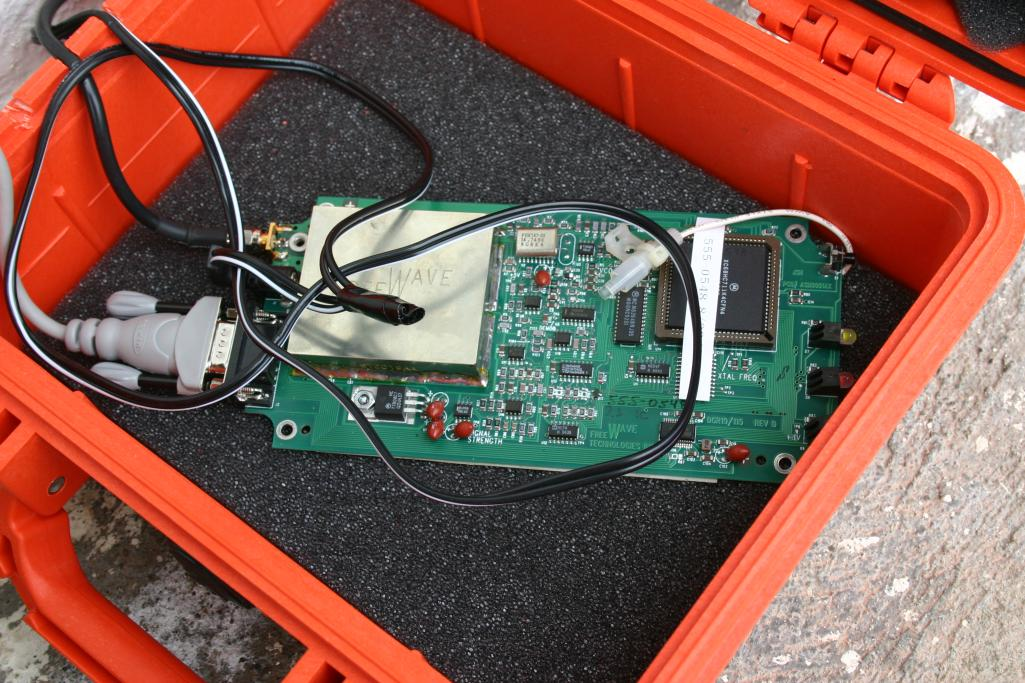
\includegraphics[height=0.1\vsize]{./figures/pics/freewave.jpg} &
%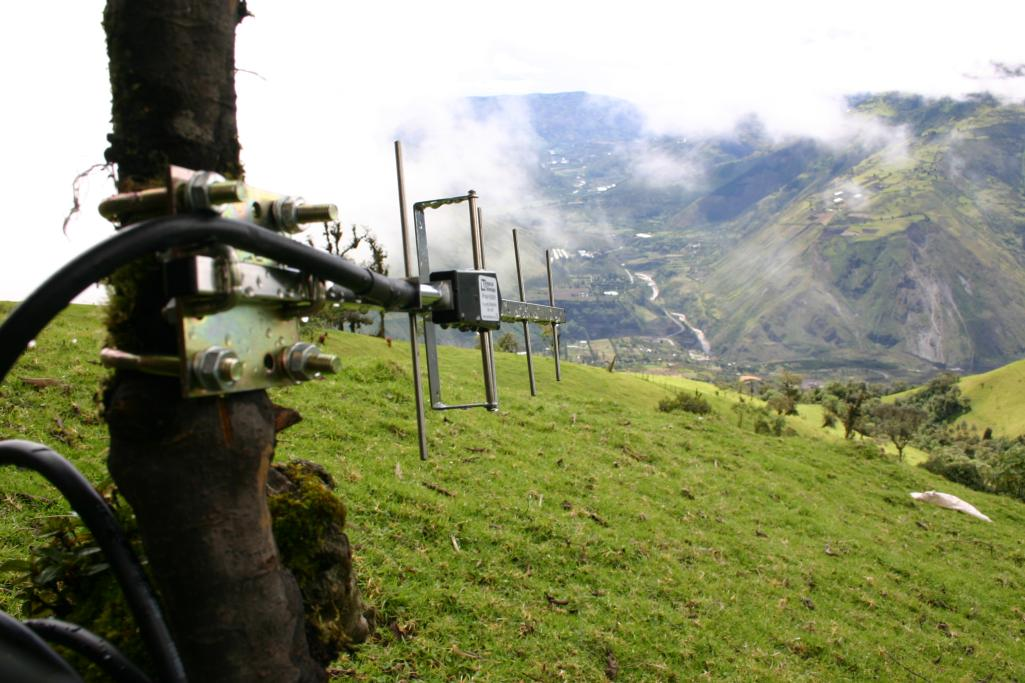
\includegraphics[height=0.1\vsize]{./figures/pics/yagi.jpg} \\
%{\small\bf (a) Infrasonic monitoring\\node.} &
%{\small\bf (b) FreeWave modem.} &
%{\small\bf (c) Yagi antenna oriented\\towards observatory.} \\
%\end{tabular}
%\end{center}
%\caption{\small {\bf Equipment used in our sensor network deployment.}}
%\label{fig-infrasound}

The infrasound monitoring node (Figure~\ref{fig-infrasound}(a)) 
uses a custom sensor board\footnote{This board was designed by 
Pratheev Sreetharan at Harvard University.}
consisting of an
amplifier and filtering circuit connected to a Panasonic WM-034BY
omnidirectional electret condenser microphone. These microphones have 
been used in other infrasonic monitoring studies~\cite{Johnson04}
and have been found to have very good low frequency response, despite
their small size. The sensor board has a manually configurable gain
setting (from 1x to 20x) using a jumper block. Given the low dynamic
range of the ADC on the Mica2 motes (10~bits), we used the highest
gain setting during our deployment. 

%\XXXnote{Need to say more about the filter and frequency response,
%etc. here}

Each infrasound node was programmed to sample data continuously at
102.4~Hz, allowing signals up to 51.2~Hz to be 
accurately.\footnote{Because the TinyOS timer component measures time in
binary milliseconds, 102.4~Hz is
the closest available value to our desired sampling frequency of 100~Hz.}
A set of 25~consecutive samples is packed into a 32-byte radio packet
and transmitted at approximately 4~Hz. The radio packet
header includes a sequence number (used to detect lost packets), the 
source node ID, and information on the most recent GPS timestamp 
(Section~\ref{sec-gps}). Upon receiving each packet, the aggregator
node transmits a short acknowledgment. If the acknowledgment is not
received by the source node, it will attempt retransmission 
up to 5~times.

After some initial experimentation with this design, we noticed that 
the samples provided by the Mica2's internal ADC were distorted
during radio transmission. While the radio is in the process of
transmitting a packet, any ADC readings taken were
offset lower by several bits. Because of the length of the radio
message, preamble, and other overhead, up to 3~samples in a given
packet may be affected by the transmission of the previous packet.
We believe this is caused by the lack of an external, fixed voltage 
reference for the ADC, some issues with the Mica2 ground plane, 
as well as EM interference from the radio oscillator itself. 
However, due to the relatively high sample rate, we were unable to 
completely avoid sampling during radio transmissions. 

\begin{figure}[t]
\begin{center}
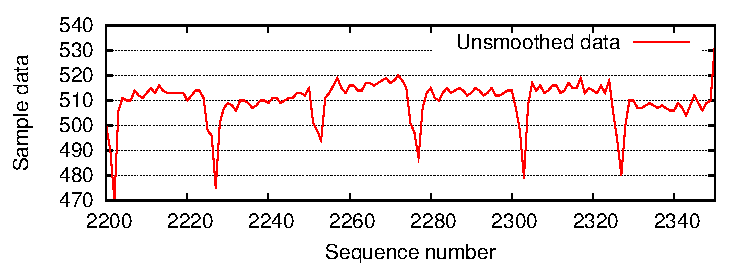
\includegraphics[width=0.9\hsize]{./figures/smooth/data-noise.pdf}  \\
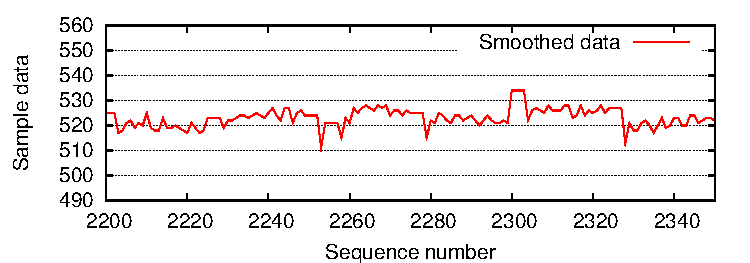
\includegraphics[width=0.9\hsize]{./figures/smooth/data-smooth.pdf}
\end{center}
\caption{\small {\bf Data filtering to correct for radio
interference with analog-to-digital signal conversion on the Mica2.} 
{\em The top figure shows an acoustic signal from
a mote before filtering; the 4~Hz noise is caused by radio
transmissions interfering with the ADC. The bottom figure shows a signal 
from a different mote with filtering enabled.}}
\label{fig-distortion}
\end{figure}

To correct this distortion, we utilized information from the TinyOS
MAC layer, which allows an application component to be notified 
when a message is being transmitted through the 
{\tt RadioSendCoordinator.startSymbol()} event. The difference
between the last ADC reading before the transmission and the first
reading during the transmission is measured. If this offset is 
below some small threshold, an offset is added to each ADC reading taken 
during transmission. While this is a very simple filter, 
it effectively corrects for the ADC distortion (Figure~\ref{fig-distortion}).

This problem motivates the need good for cross-layer information flow 
in embedded systems software. The application's ability to know
exactly which ADC readings are affected by a radio transmission allows
the data to be corrected on the fly, rather than attempting to
correct the signal distortion after the fact.
However, better hardware designs are another solution: our initial testing 
of the Moteiv Telos motes~\cite{telos} indicates that they do not exhibit
this problem.

\subsection{Aggregator node and long-distance data transmission}

The aggregator node receives infrasonic sample and GPS timestamp 
messages and acknowledges them, as described above. It 
relays each received message to its serial port, which is connected 
to a FreeWave spread-spectrum modem (Figure~\ref{fig-infrasound}(b)) providing
a reliable serial data connection over distances of 20~km or more. 
On the receiving end of the link, a second FreeWave modem is connected to a
laptop base station running a Java program that logs the raw data to a series
of files. Each file contains the raw contents of each
received radio packet, consisting of infrasound samples from each
sensor node as well as GPS timestamp messages (see below). The
real-time data is also exported via a TCP socket (using the TinyOS
{\em serialforwarder} program) to allow other programs to visualize 
or process the stream of samples in real time. 
All other data analysis was performed on the logged data files.

\subsection{GPS receiver node}
\label{sec-gps}

Because we are interested in correlating signals across multiple
sensor nodes and comparing our signals to those captured at
co-located wired sensor arrays, it is essential that we
accurately timestamp the sensor data from each
node. For this purpose, we made use of a Garmin GPS~18LVC receiver
puck that provides a 1~Hz digital signal accurate 
to within 1~$\mu$sec of the GPS timebase, through a serial
interface transmitting binary or ASCII~NMEA~0183 GPS data.
The GPS puck is connected to a separate Mica2 node acting as a GPS
receiver, with the PPS time signal tied to an interrupt line.

Our time synchronization protocol is similar in nature to
RBS~\cite{elson-rbs}. When the PPS interrupt from the GPS receiver 
is raised, the GPS receiver node records the local value of a 921.6~KHz 
timer. It then broadcasts a radio packet containing a sequence number,
the GPS timestamp of the {\em previous\/} NMEA~0183 GGA sentence in
$HHMMSS$ format, and the delay (measured in ticks from the 921.6~KHz
timer) between the PPS interrupt and the time that the node begins
transmitting the message (that is, after MAC delay and backoff).

Because every sensor node will receive this radio message at the same
time, we can record the local time at each node when this message was
received and use this information to cross-correlate the
signals being captured by each infrasound node.
The MAC delay reported by the GPS sender can be used to register this 
common timebase back to the true GPS time for comparison with other
stations. Our initial deployment only requires single-hop time 
synchronization, although this approach can be readily extended to multihop
cases using a multihop time synchronization 
protocol~\cite{vanderbilt-flooding}.

\subsection{Time regression}
\label{sec-regression}

To perform analysis of the data recorded across the sensor array, it
is necessary to align the sample streams from each node to a common
timebase. This step is performed offline on the data logged at
the base station. Each log entry consists of a tuple of the form
{\em \{moteid, packetno, sample\}}, where {\em moteid} is the ID of the 
transmitting mote, {\em seqno} is the sequence number for the 
corresponding radio packet, and {\em sample} is
the 10-bit ADC sample data. Recall that 25~samples are contained in each
radio message. If a GPS timestamp message was received by
the node while collecting samples in this packet, the log entry 
will also contain two additional fields: the sequence number of the
GPS timestamp message, and the index of the sample (0~to~24) that 
was being acquired when the GPS message was received.
The true GPS time and transmission delay for each GPS timestamp is
logged separately.

%Using this information it is possible to align the signals to a 
%common timebase. 
We expect that the sampling rate of individual
nodes may vary slightly over time, due to changes in temperature 
and battery voltage. In addition, our logs do not record the precise
time that a GPS timestamp message arrives during the acquisition of
a sample. To address these uncertainties, we apply a linear regression 
to the logged data stream, using the samples tagged with GPS timestamp
arrivals as inputs to the regression. The output is the estimated 
sampling rate of each node over time, allowing individual samples to
be mapped to a ``true'' time that the sample was acquired.
The regression is applied to runs of logged samples with no more than
100 missing packets between runs, and with a maximum of 10,000 samples
in each run. 

\subsection{Physical packaging}

Clearly, leaving sensor nodes in an exposed environment requires
appropriate physical packaging to protect the instruments from
moisture, humidity, and sunlight. Our nodes were enclosed in watertight 
Pelican cases of various sizes, which are inexpensive, easy to open and 
close, and very effective at protecting against the elements. 
Weatherproof 1/4-wave whip antennas were used for each of the sensor 
nodes, which were attached to the outside of each Pelican case, and a
small hole was drilled to thread the antenna pigtail inside the case.
Silicone sealant was used to weatherproof this opening.

The microphones require open access to the atmosphere to
measure incident pressure waves from the volcano.  A small hole was 
drilled on the side of the infrasonic microphone node cases to allow
approximately 1~m of coax cable attaching the microphone 
to the mote inside the case. The microphones themselves were protected
with a makeshift wind- and rain-shield consisting of the top cut off
of a two-liter plastic pop bottle. The microphone was placed inside
the mouth of the bottle and oriented downwards to minimize moisture
accumulation.

